\documentclass[12px]{article}
\usepackage[cjk]{kotex}
\usepackage[top=2cm, bottom=2cm, left=2.5cm, right=2.5cm]{geometry}
\usepackage{amsmath, amssymb}
\usepackage{enumerate}
\usepackage{graphicx}

\everymath{\displaystyle}

\title{응용통계학 10장 연습문제 풀이}
\author{20181653 이강희}
\date{}

\begin{document}
\maketitle

\begin{center}
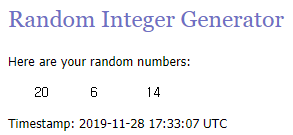
\includegraphics[scale=0.7]{random}
\end{center}

\section*{6번}
- 귀무가설 $H_0 : \mu = 100$ \\
- 대립가설 $H_1 : \mu > 100$ \\
- 유의수준 $\alpha = 0.01$ \\
- 기각역 $z > z_{0.01} = 2.33$ \\
- 검정통계량 $z = \frac{106-100}{35/\sqrt{100}} \approx 1.714$ \\
- 귀무가설 $H_0$ 채택

\section*{14번}
- 귀무가설 $H_0 : p = 0.92$ \\
- 대립가설 $H_1 : p > 0.92$ \\
- 유의수준 $\alpha = 0.05$ \\
- 기각역 $z > z_{0.05} = 1.645$ \\
- 검정통계량 $z = \frac{153-165 \times 0.92}{\sqrt{165 \times 0.92 \times 0.08}} \approx 0.344$ \\
- 귀무가설 $H_0$ 기각

\section*{20번}
- 귀무가설 $H_0 : \sigma^2 = 300$ \\
- 대립가설 $H_1 : \sigma^2 \neq 300$ \\
- 유의수준 $\alpha = 0.05$ \\
- 기각역 $\chi^2 < \chi_{1-0.025}^{2} = 73.3661$ 또는 $\chi^2 > \chi_{0.025}^{2} = 128.422 \ (\nu=99)$ \\
- 검정통계량 $\chi^2 = \frac{99 \times 220}{300} = 72.6$ \\
- 귀무가설 $H_0$ 기각

\end{document}

